
\section{Codebeispiele}
\subsection{Risikokarte}
\begin{figure}[H]
  \centering
  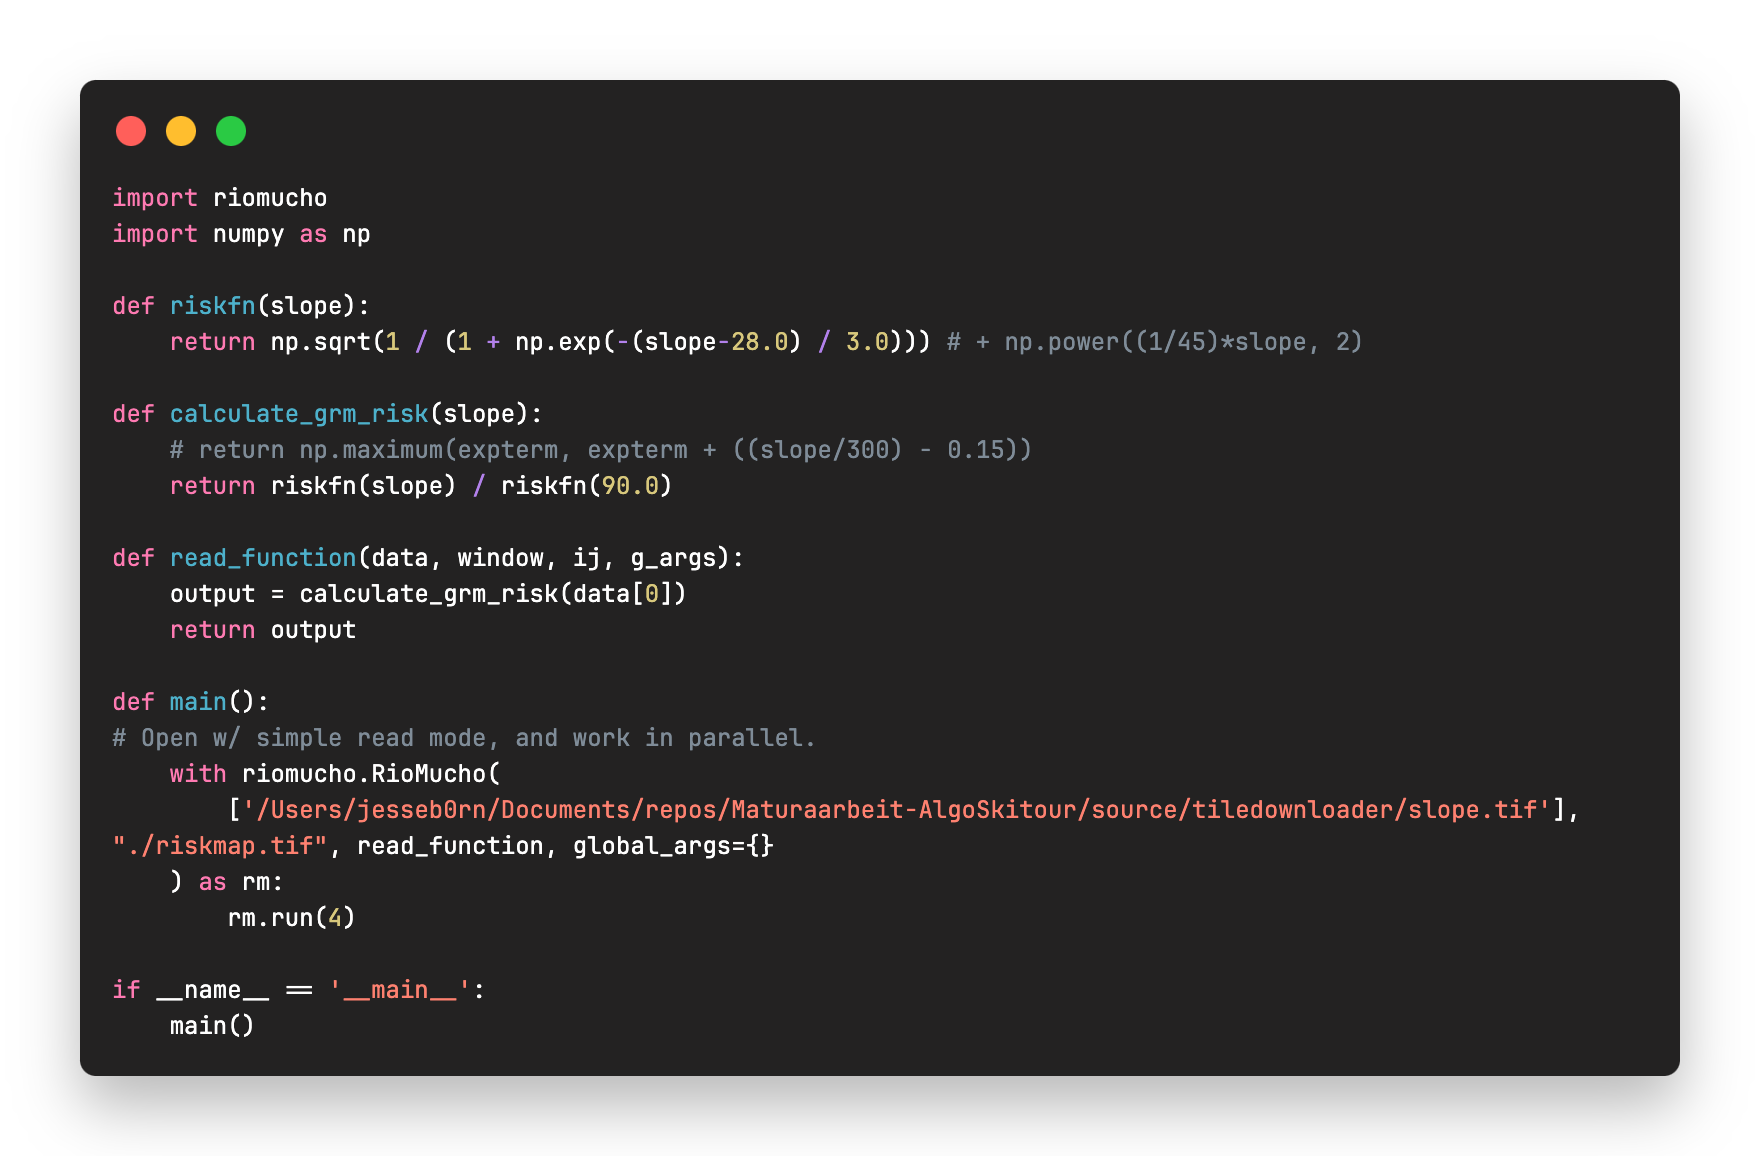
\includegraphics[width=0.9\linewidth]{code}
  \caption{Python Code zur Produktion von Risikokarten aus Neigungskarte}\label{fig:python}
\end{figure}

\section{Evaluationsrouten}\label{app:evalroutes}

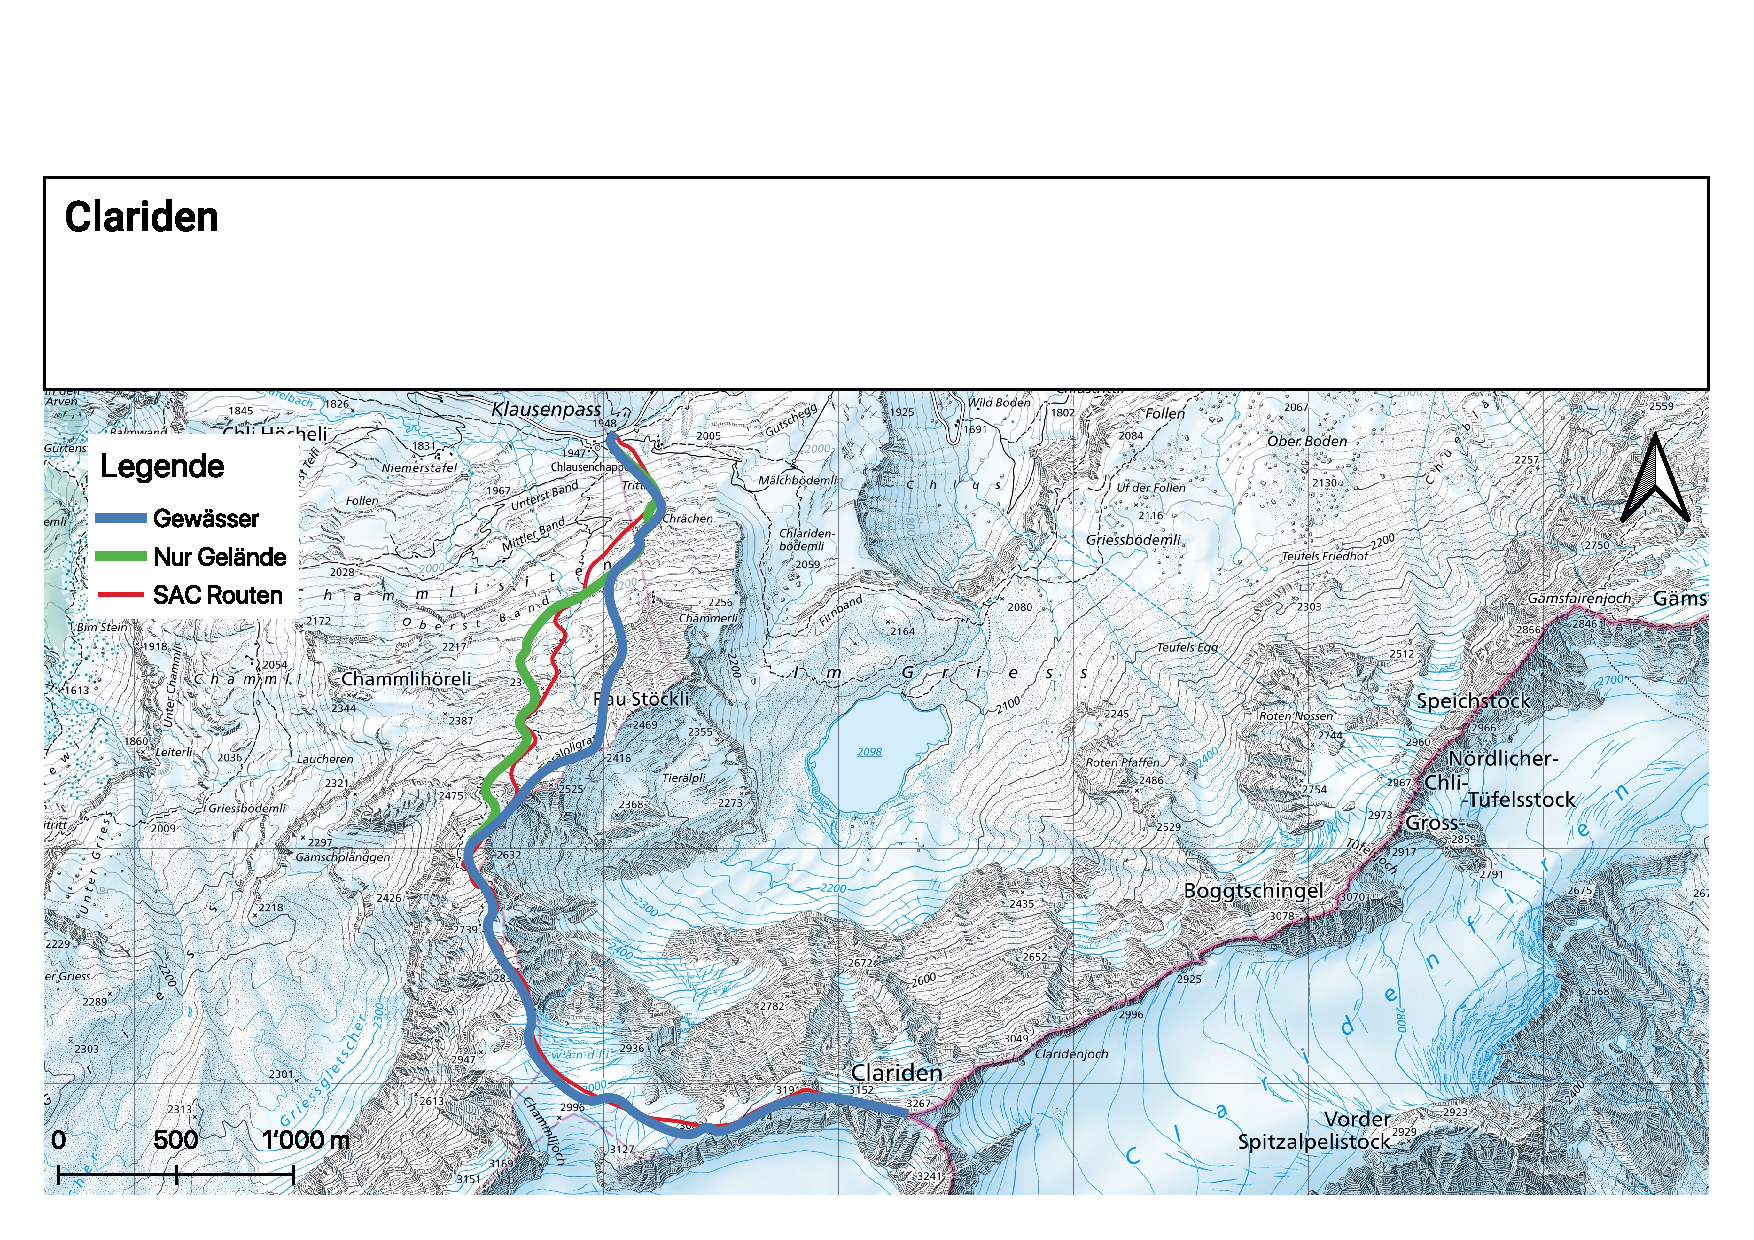
\includepdf[landscape=true]{./../evaluation/PDFs/Clariden.pdf}
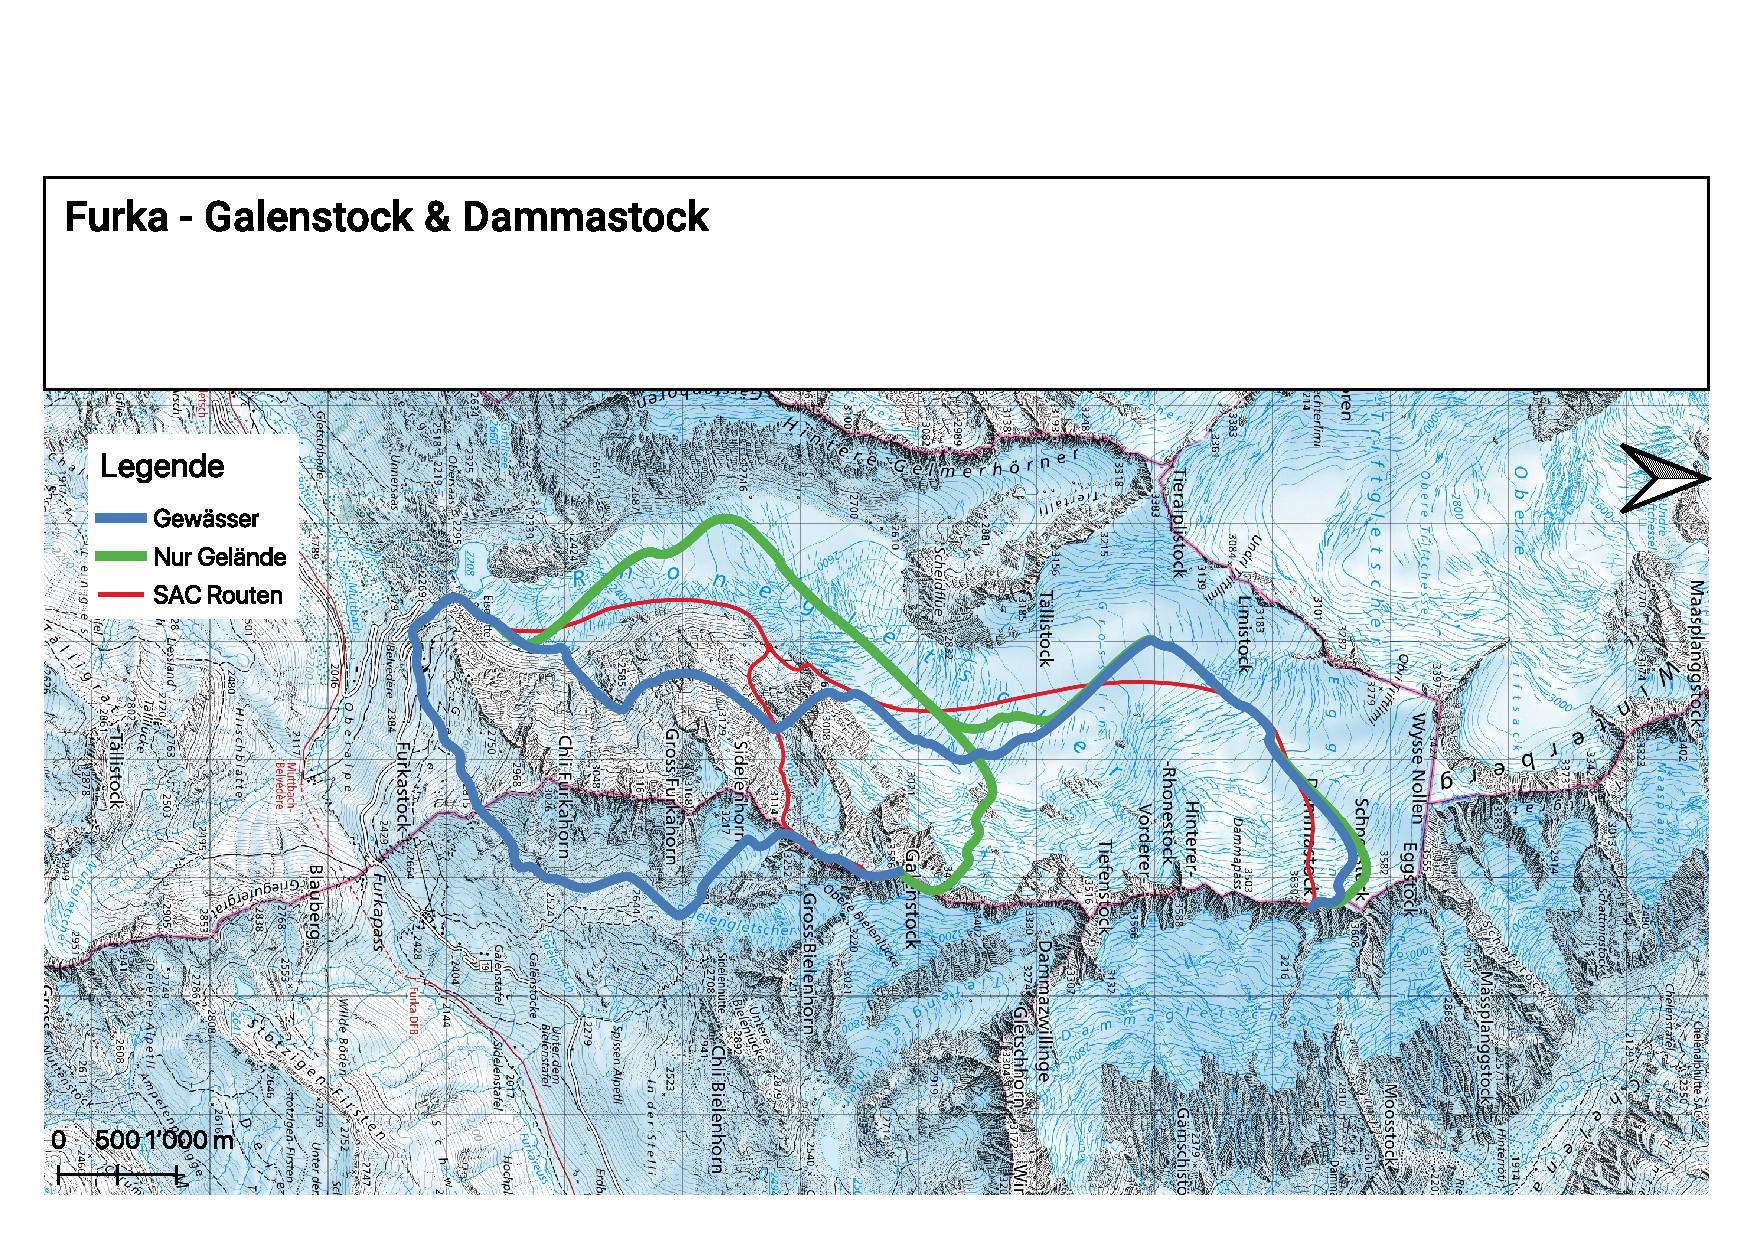
\includepdf[landscape=true]{./../evaluation/PDFs/Furka - Galenstock & Dammastock.pdf}
\includepdf[landscape=true]{./../evaluation/PDFs/Länta - Rheinwaldhorn_Adula.pdf}
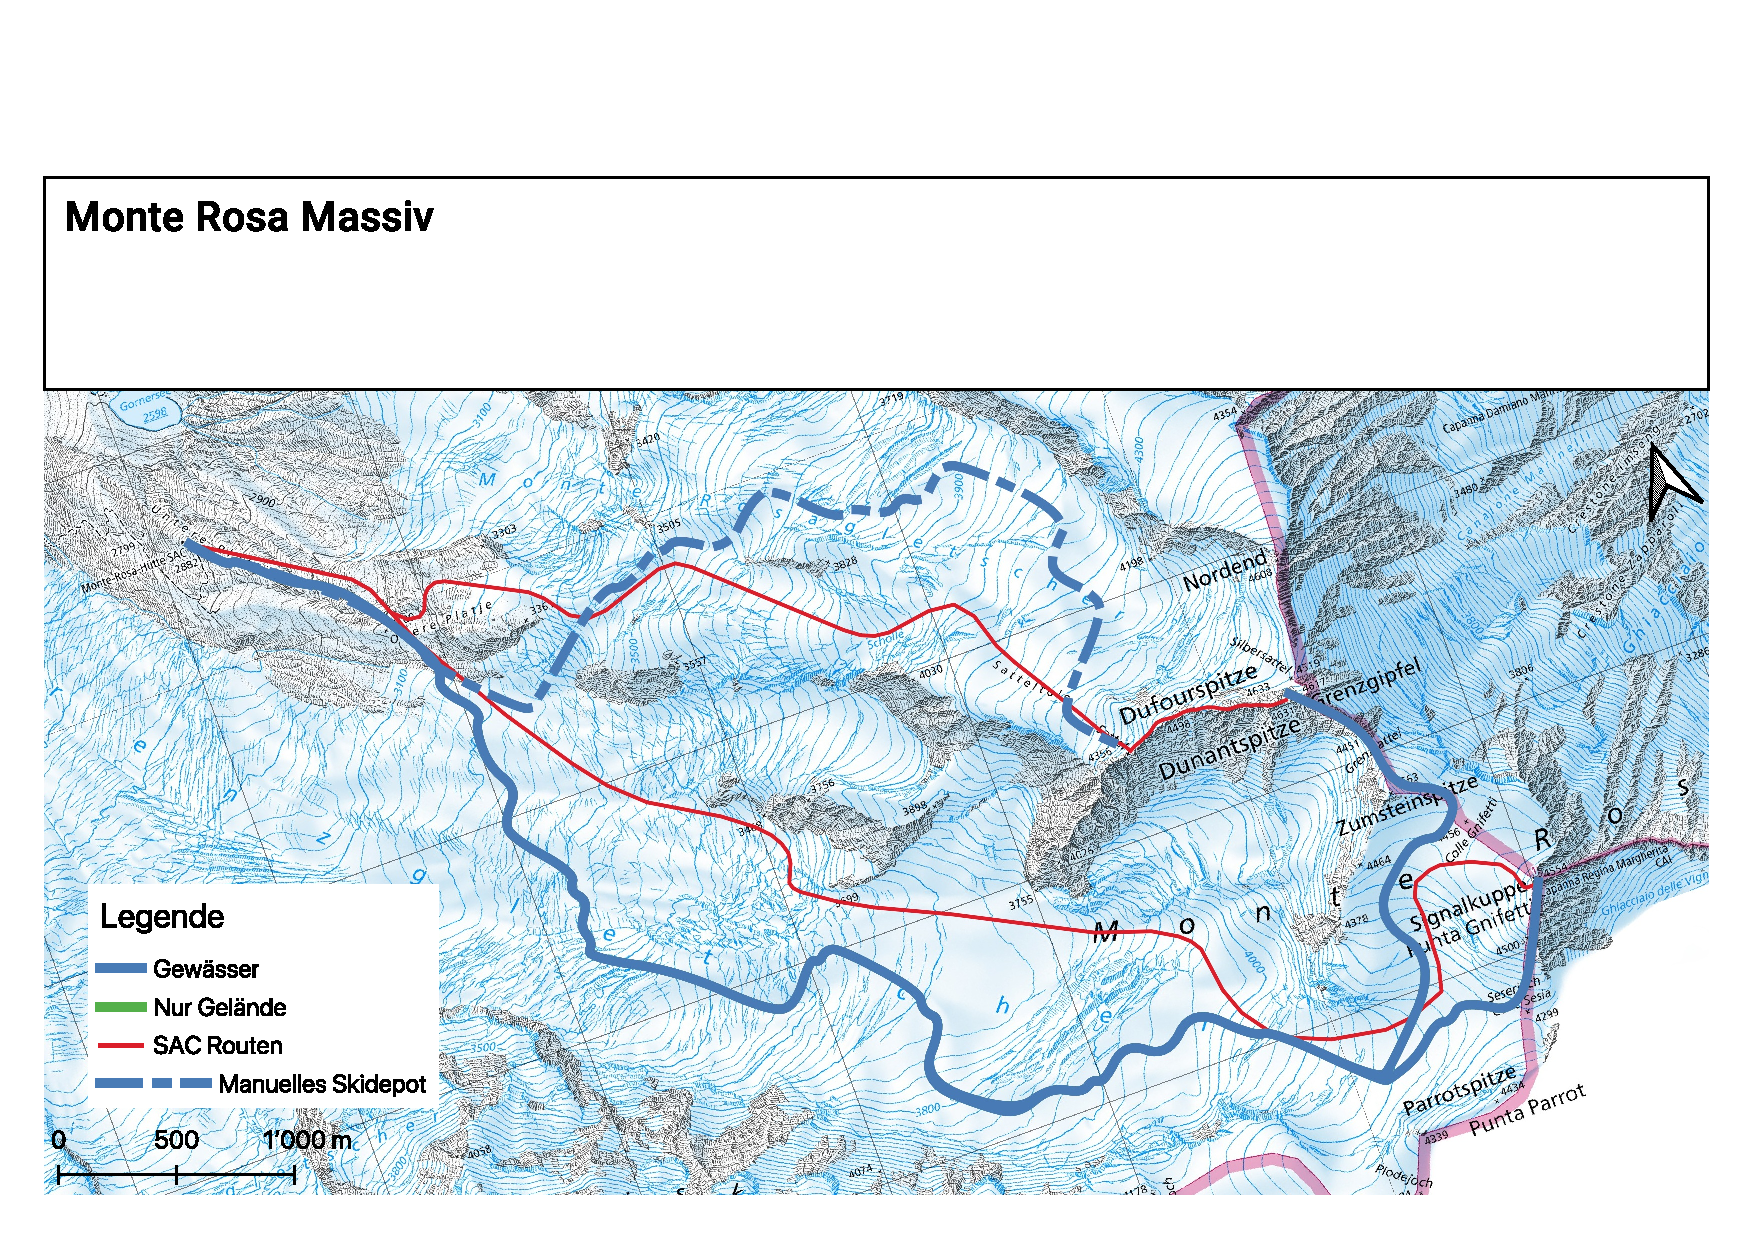
\includepdf[landscape=true]{./../evaluation/PDFs/Monte Rosa Massiv.pdf}
\includepdf[landscape=true]{./../evaluation/PDFs/Piz Palü.pdf}
\includepdf[landscape=true]{./../evaluation/PDFs/Strahlhorn.pdf}
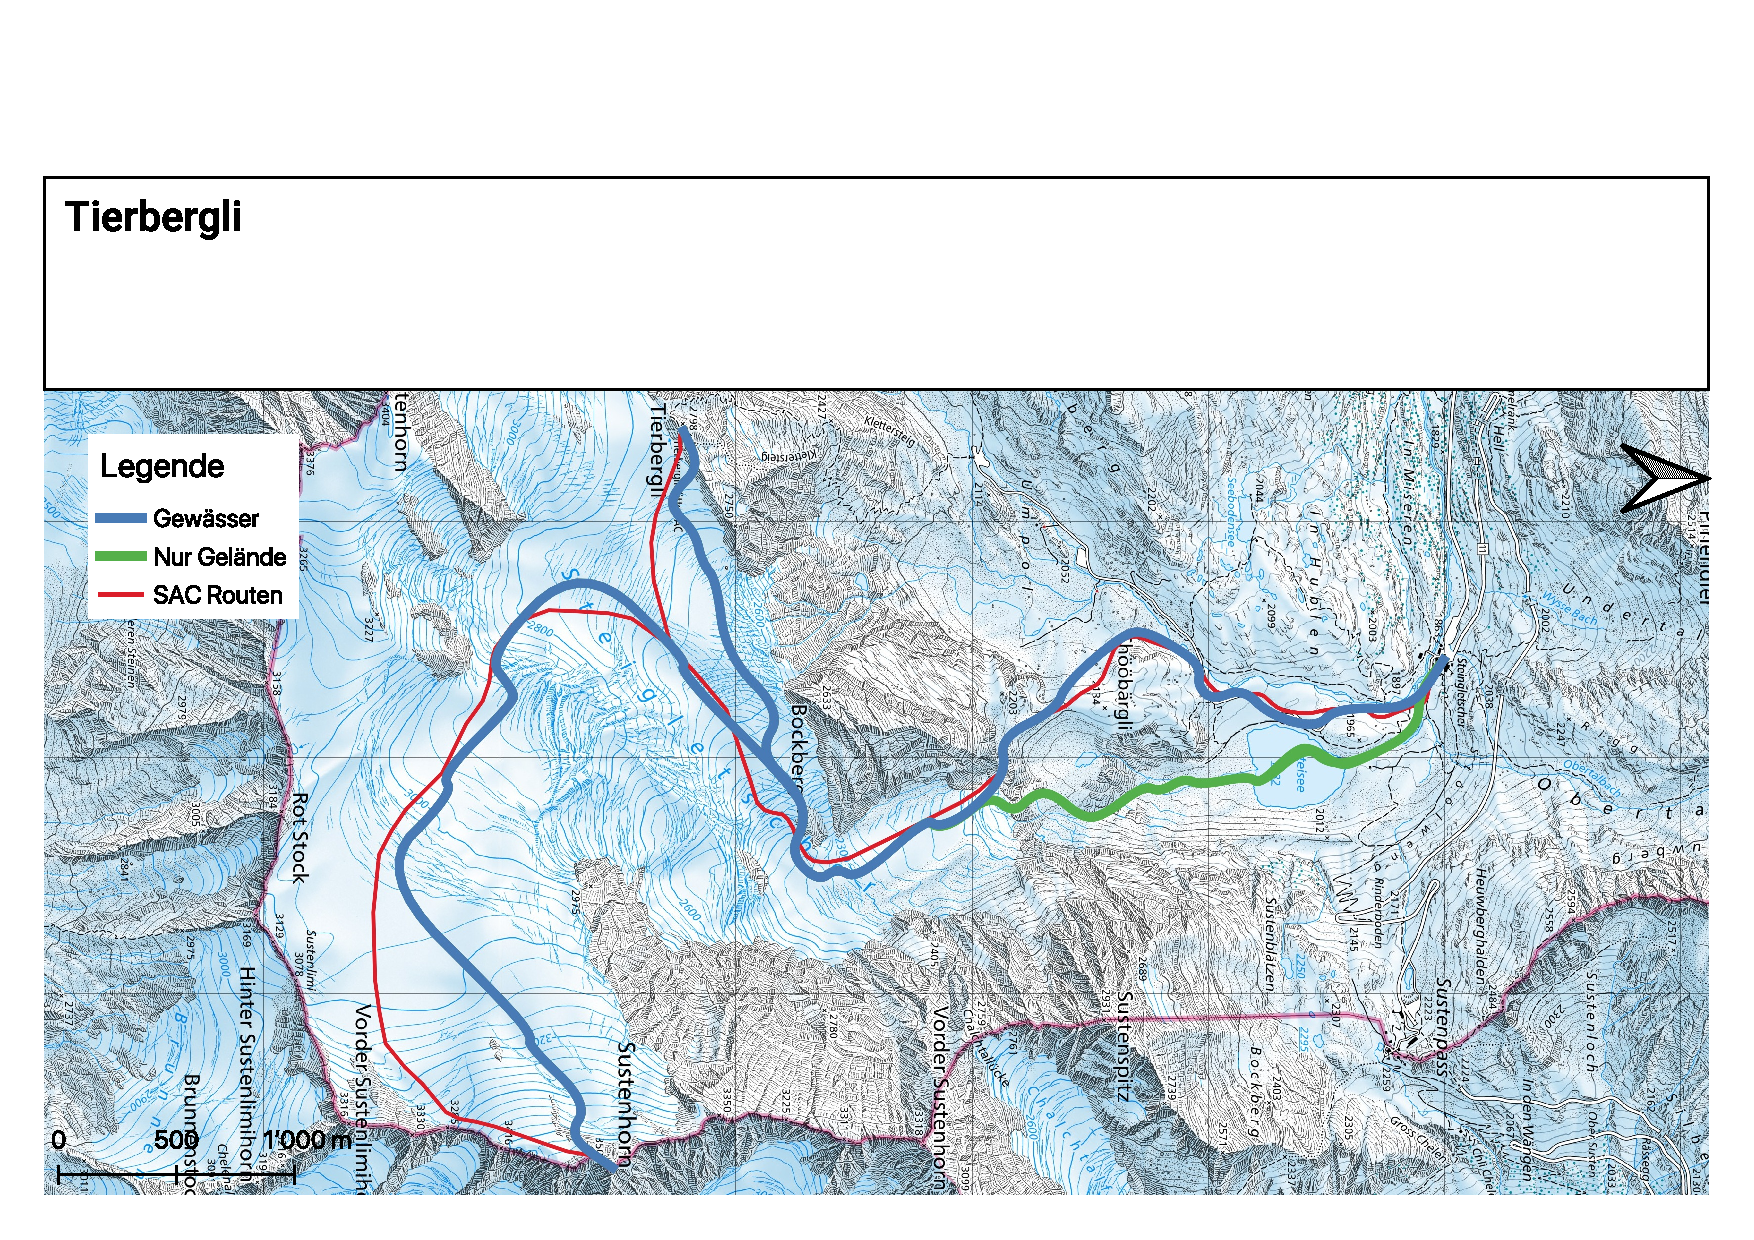
\includepdf[landscape=true]{./../evaluation/PDFs/Tierbergli.pdf}

\section{Lawinensimulation mit \\RAMMS::Avalanche}
\section{It's not a bug, it's a feature}